\textcolor{red}{This section should present the obtained results and provide an insightful analysis of them. You can present the results using graphs, tables, or any other visualization method suits your purpose. Do not forget to include proper captions \cite{zobel2014graphs} in any of these illustration methods you use. You do not need to provide any execution details as they are already presented in Sec.~\ref{sec:experimentation}.}

\textcolor{red}{A good practise would be to compare your algorithm with a simpler approach, such as (a) a naive method, (b) a Hill Climbing approach, or (c) a simple evolutionary algorithm. In the third case, you can use the simpler version of the algorithm you developed, i.e., the original algorithm without your modifications. In that case, you should briefly describe the comparing method(s) in Sec.~\ref{sec:experimentation}. Alternatively, you can use some reference results derived from the repositories you found some benchmark instances.}

\textcolor{red}{To display tables, the \texttt{booktabs} package might be useful. For example, Table~\ref{tab:results_example} shows how you should increase the  size of $n$, when running your code. You can advice \cite{zobel2014graphs} to see a few examples of proper tables.}

\begin{table}[h]
	\centering
	\caption{Example of comparison the developed algorithm's results with the best ones from a repository.}
	\label{tab:results_example}
	\begin{tabular}{lrrr}
		\toprule
		\textbf{Instance} & \textbf{Optimum (Repository xyz)} & \textbf{EA} & \textbf{time (s)} \\
		\midrule
		st70              & 678.597                           & 677.109     & 0.67              \\
		ei176             & 545.387                           & 544.369     & 1.16              \\
		kroA100           & 21285.443                         & 21285.443   & 1.69              \\
		rd100             & 7910.396                          & 7910.396    & 2.14              \\
		Pr136             & 96772                             & 96770.924   & 7.11              \\
		Pr144             & 58537                             & 58535.221   & 7.97              \\
		a280              & 2856.769                          & 2856.769    & 33.47             \\
		\bottomrule
	\end{tabular}
\end{table}

\textcolor{red}{You can use different illustration methods to present different aspects of your analysis. Figure~\ref{fig:plot_example} gives an example using the \href{https://www.overleaf.com/learn/latex/Pgfplots_package}{\texttt{pgfplots}} package.}

\begin{figure}[h]
	\centering
	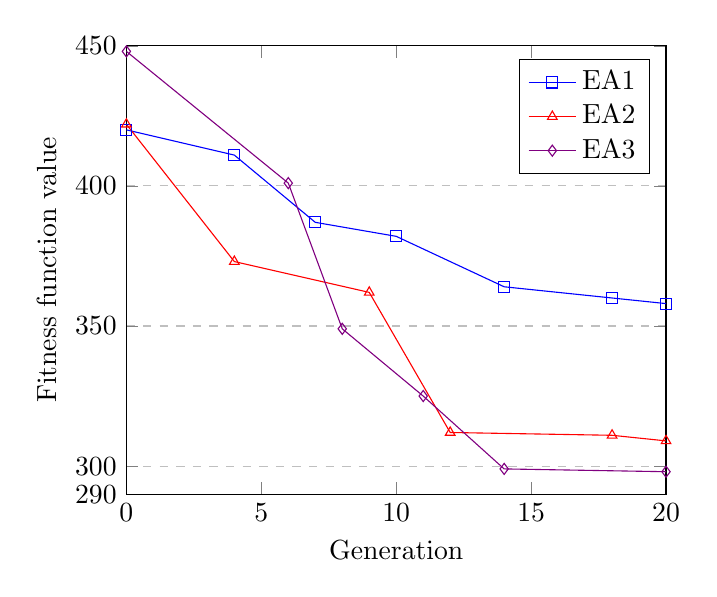
\begin{tikzpicture}
		\begin{axis}[
				% title={Example of convergence analysis},
				xlabel={Generation},
				ylabel={Fitness function value},
				xmin=0, xmax=20,
				ymin=290, ymax=450,
				xtick={0,5,10,15,20},
				ytick={290,300,350,400,450},
				legend pos=north east,
				ymajorgrids=true,
				grid style=dashed,
			]

			\addplot[
				color=blue,
				mark=square,
			]
			coordinates {
					(0,420)(4,411)(7,387)(10,382)(14,364)(18,360)(20,358)
				};
			\addlegendentry{EA1}

			\addplot[
				color=red,
				mark=triangle,
			]
			coordinates {
					(0,422)(4,373)(9,362)(12,312)(18,311)(20,309)
				};
			\addlegendentry{EA2}

			\addplot[
				color=violet,
				mark=diamond,
			]
			coordinates {
					(0,448)(6,401)(8,349)(11,325)(14,299)(20,298)
				};
			\addlegendentry{EA3}

		\end{axis}
	\end{tikzpicture}
	\caption{Example of convergence analysis.}
	\label{fig:plot_example}
\end{figure}

\lipsum[4]